\documentclass[a4paper,11pt]{article}
\usepackage{graphicx}
\usepackage{float}
\usepackage{subfig}
\usepackage{geometry}
\usepackage{amsmath,amssymb}
\usepackage{amsthm}
\usepackage{bbold}
\usepackage{mathtools}
\usepackage{braket}
\usepackage{booktabs}
\usepackage[table,xcdraw]{xcolor}
\usepackage[utf8]{inputenc}
\usepackage{cite}
\usepackage[english]{babel}
\usepackage{lipsum}
\usepackage{setspace}
\usepackage{minted}
\usepackage{xcolor}
\newcommand{\R}{\mathbb{R}}
\usepackage{hyperref}
\hypersetup{colorlinks=true,linkcolor=blue}
\geometry{a4paper, top=2.5cm, bottom=2.5cm, left=3cm, right=2.5cm}

\begin{document}
	\author{Catalano Giuseppe, Cerrato Nunzia}
	\title{Numerical Linear Algebra Homework Project 4:\\Unconstrained Optimization}
	\date{}
	\maketitle
	
	\noindent In this project we want to perform unconstrained optimization using the Newton method both in its standard form and by considering its variants which make use of the backtracking and the trust region approach.
	The first function that we report is called \mintinline{Python}{Newton} and it performs the standard Newton algorithm, with the possibility of using backtracking for the choice of $\alpha$ if \mintinline{Python}{backtracking=True} is passed as a keyword argument to the function. The second function is called \mintinline{Python}{Newton_trust_region} and it performs the Newton algorithm with the trust region approach. These two functions are presented with their documentation and they can be found in the library \mintinline{Python}{Project_4.py} on \href{https://github.com/nunziacerrato/Numerical_Analysis_Optimization/blob/main/Project_4/Project_4.py}{GitHub}.
	We will apply these methods to four test functions and, in some cases, we will compare these approaches to see how convergence changes.
	
\section{Algorithms}
\begin{minted}[mathescape, linenos, breaklines]{python}
def Newton(func, grad, hess, tol, maxit, x_0, sol_x, sol_f, alpha=1, sigma=0.0001, rho=0.5, backtracking=False):
    r''' This function implements the standard Newton method for unconstrained optimization.

     Parameters
     ----------
     func : function
         Function to be minimized. It must be :math:`f : \mathbb{R}^{n} \rightarrow \mathbb{R}`
     grad : function
         Gradient of the function. It returns a 1d-array (vector)
     hess : function
         Hessian of the function. It returns a 2d-array (matrix)
     tol : float
         Tolerance parameter for the stopping criterion
     maxit : int
         Maximum number of iterations
     x_0 : ndarray
         Starting point
     sol_x : ndarray
         Exact solution (x) to the minimization problem
     sol_f : float
         Exact minimum value of the function
     alpha : float
         Step lenght. Default value alpha=1
     sigma : float
         Constant parameter in :math:`(0,1)`. Used if backtracking = True. Default value sigma=0.0001
     rho : float
         Reduction parameter in :math:`(0,1)`. Used if backtracking = True. Default value rho=0.5

     Results
     -------
     results : dict
         Dictionary of the results given by the function. It contains the following items:
           - 'convergence' : (bool) True if the algorithm converges, False if it doesn't converge
           - 'k' : (int) final iteration at which convergence is reached
           - 'min_point' : (ndarray) computed point at which the minimum of the function is reached
           - 'min_value' : (float) computed minimum value of the function
           - 'interm_point' : (list) list of the intermediate points
           - 'error_x' : (list) list that contains the 2-norm of the difference between each intermediate point and the exact solution (min_point). 
           - 'error_f' : (list) list that contains the difference between the function evaluated at each intermediate point and its value in the exact minimum point
           - 'scalar_product' : (list) list that contains the scalar product between the descent direction and the gradient

     '''
    old_point = x_0
    alpha_0 = alpha

    # Create a list to save intermediate points
    interm_points = [old_point]
    # Create a list to save the scalar product between the gradient and the descent direction
    scalar_prod = []

    new_point = x_0 
    norm_diff_x = np_lin.norm(new_point - old_point)
    # Cycle on the number of iterations
    for k in range(maxit):
        gradient = grad(old_point)
        hessian = hess(old_point)

        # Compute norms for the stopping criterion
        norm_grad = np_lin.norm(gradient)

        # Check if the stopping criterion is satisfied
        if norm_grad <= tol and norm_diff_x <= tol*(1 + np_lin.norm(old_point)):            
            min_value = func(new_point)
            conv = True
            break

        # Compute the descent direction by solving a linear system
        p = np_lin.solve(hessian, -gradient)
        scalar_prod.append(gradient@p)

        # Implement backtracking if backtracking == True
        if backtracking == True:
            alpha = alpha_0
            iteraz_backtracking = 0 
            while func(old_point + alpha*p) > func(old_point) + (sigma*alpha)*(p @ gradient) and iteraz_backtracking < 100:
                alpha = rho*alpha
                iteraz_backtracking += 1         

        # Compute the new point and add it to the list of intermediate points
        new_point = old_point + alpha*p
        interm_points.append(new_point)
        norm_diff_x = np_lin.norm(new_point - old_point)

        old_point = new_point

    if k == maxit-1:
        min_value = func(new_point)
        conv = False

    gradient = grad(new_point)
    hessian = hess(new_point)
    p = np_lin.solve(hessian, -gradient)
    scalar_prod.append(gradient@p)

    # Compute the 2norm of the difference between each intermediate point and the exact solution
    error_x = [np_lin.norm(interm_x - sol_x) for interm_x in interm_points]

    # Compute the difference between the function evaluated in each intermediate point and its value in the exact minimum point
    error_f = [func(interm_x) - sol_f for interm_x in interm_points]

    results = {'convergence': conv, 'k' : k, 'min_point' : new_point, 'min_value' : min_value , 'interm_point' : interm_points, 'error_x' : error_x, 'error_f' : error_f, 'scalar_product' : scalar_prod}

    return results

\end{minted}

\noindent Below the code of the trust region Newton algorithm.


\begin{minted}[mathescape, linenos, breaklines]{python}
def Newton_trust_region(func, grad, hess, tol, maxit, x_0, sol_x, sol_f, alpha=1, eta=0.01):
    ''' This function implements the Newton method with the trust region approach for unconstrained optimization.

    Parameters
    ----------
    func : function
        Function to be minimized. It must be :math:`f : \mathbb{R}^{n} \rightarrow \mathbb{R}`.
    grad : function
        Gradient of the function. It returns a 1d-array (vector)
    hess : function
        Hessian of the function. It returns a 2d-array (matrix)
    tol : float
        Tolerance parameter for the stopping criterion
    maxit : int
        Maximum number of iterations
    x_0 : ndarray
        Starting point
    sol_x : ndarray
        Exact solution (x) to the minimization problem
    sol_f : float
        Exact minimum value of the function
    alpha : float
        Step lenght. Default value alpha=1
    eta : float
        Constant parameter in :math:`(0,0.25)`. Default value eta=0.01
        
    Results
    -------
    results : dict
        Dictionary of the results given by the function. It contains the following items:
          - 'convergence' : (bool) True if the algorithm converges, False if it doesn't converge
          - 'k' : (int) final iteration at which convergence is reached
          - 'min_point' : (ndarray) computed point at which the minimum of the function is reached
          - 'min_value' : (float) computed minimum value of the function
          - 'interm_point' : (list) list of the intermediate points
          - 'error_x' : (list) list that contains the 2-norm of the difference between each intermediate point and the exact solution (min_point). 
          - 'error_f' : (list) list that contains the difference between the function evaluated at each intermediate point and its value in the exact minimum point
          - 'scalar_product' : (list) list that contains the scalar product between the descent direction and the gradient
    '''

    # Evaluate the gradient and the hessian in the starting point
    gradient = grad(x_0)
    hessian = hess(x_0)

    # Compute the first descent direction and the first delta value
    p = np_lin.solve(hessian, -gradient)
    delta = np_lin.norm(p)

    interm_points = [x_0]
    scalar_prod = []
    old_point = x_0

    # Cycle on the number of iterations
    for k in range(maxit):

        # Evaluate the gradient and the hessian at the current point
        gradient = grad(old_point)
        hessian = hess(old_point)

        # Diagonalize the hessian computed at the current point
        eigval, eigvect = np_lin.eigh(hessian)
        # Choose an initial mu value
        mu = abs(min(min(eigval), 0)) + 1e-12
        coeff_vect = eigvect.T @ gradient/(eigval + mu)

        # Choose the optimal mu value which respects the condition on the 2-norm
        while sum([coeff**2 for coeff in coeff_vect]) > delta**2:
            mu = mu*2
            coeff_vect = eigvect.T @ gradient/(eigval + mu)

        # Compute the descent direction
        p = - eigvect @ coeff_vect
        scalar_prod.append(- gradient @ eigvect @ np.diag(1/eigval) @ eigvect.T @ gradient)

        new_point = old_point + alpha*p

        # Choose the value of delta for the successive iteration
        rho = (func(new_point)-func(old_point))/(p @ gradient + 0.5*p @ hessian @ p)

        if 0 < rho < 0.25:
            delta = delta/4
        elif rho > 0.75:
            delta = 2*delta
        elif 0 < rho < eta:
            new_point = old_point
        
        interm_points.append(new_point)

        # Compute norms for the stopping criterion
        norm_grad = np_lin.norm(gradient)
        norm_diff_x = np_lin.norm(new_point - old_point)

        # Check if the stopping criterion is satisfied
        if norm_grad <= tol and norm_diff_x <=tol*(1 + np_lin.norm(new_point)):
            min_value = func(new_point)
            conv = True
            break

        old_point = new_point

    if k == maxit-1:
        min_value = func(new_point)
        conv = False

    gradient = grad(new_point)
    hessian = hess(new_point)
    p = np_lin.solve(hessian, -gradient)
    scalar_prod.append(- gradient @ eigvect @ np.diag(1/eigval) @ eigvect.T @ gradient)
    
    # Compute the 2norm of the difference between each intermediate point and the exact solution
    error_x = [np_lin.norm(interm_x - sol_x) for interm_x in interm_points]

    # Compute the difference between the function evaluated in each intermediate point and 
    # its value in the exact minimum point
    error_f = [func(interm_x) - sol_f for interm_x in interm_points]

    results = {'convergence': conv, 'k' : k, 'min_point' : new_point, 'min_value' : min_value, 'interm_point' : interm_points, 'error_x' : error_x, 'error_f' : error_f, 'scalar_product' : scalar_prod}

    return results
\end{minted}


	\section{Test Functions}
	We will consider four test functions, which will be distinguished by using an apex $(a)$, $(b)$, $(c)$, $(d)$, respectively. For each of these functions, we will try to minimize it first by using the standard Newton algorithm and, if it does not converge, we will try to use backtracking or, as a last attempt, the trust region approach.\\
	
	\noindent In all of these cases, we have chosen as tolerance parameter  \mintinline{Python}{tol=1e-12} and as the maximum number of iterations allowed \mintinline{Python}{maxit=100}. Moreover, we have chosen \mintinline{Python}{alpha=1} as default $\alpha$ value and \mintinline{Python}{sigma=0.0001} and \mintinline{Python}{rho=0.5} as default parameters for backtracking. Finally, in the case of the Newton trust region method, we have chosen \mintinline{Python}{eta=0.01}. However, these constants can be passed as keyword arguments to the appropriate functions, therefore one can change their value in the main program, where these functions are effectively used.\\
	
	\noindent For each case we will report a table with the required values in correspondence with the intermediate points \footnote{Note that $k=0$ will correspond to the starting point.}, namely $\| \textbf{x}_{k} - \textbf{x}^*\|_{2} $, $f(\textbf{x}_{k}) - f(\textbf{x}^{*}) $, and $-\nabla f(\textbf{x}_{k})^{T} [\nabla^{2}f(\textbf{x}_{k})]^{-1} \nabla f(\textbf{x}_{k})$, where $\textbf{x}_{k}$ is the computed point at step $k$, $\textbf{x}^*$ is the exact minimum point, while the last term represents the scalar product between the gradient of the function and the descent direction at step $k$. We will expect the first two terms to get smaller and smaller as the algorithm approaches the minimum point, while we will expect the third one to be negative in order to have a descent direction. Values of these terms different from the expected ones might be an indication of the non-convergence of the algorithm. Finally, we will report a contour plot and a 3D plot to show how the minimum point is reached.
	
	
	\subsection{Test function (a)}
	Consider the function $f^{(a)}: \R^{2}\rightarrow \R$, defined as
	\begin{equation}
		f^{(a)}(x_{1},x_{2}) = (x_{1}-2)^{4} + (x_{1}-2)^{2}x_{2}^{2} + (x_{2}+1)^{2}.
	\end{equation}
	It is possible to note that this function assumes a minimum value $f^{(a)}(\textbf{x}^*)=0$ in correspondence with the point $\textbf{x}^*=(2,-1)$. We would like to obtain this minimum value and the corresponding point $\textbf{x}^*$ by using the standard Newton algorithm implemented by the function \mintinline{Python}{Newton}. We report below the gradient and the Hessian of $f^{(a)}(\textbf{x})$, which must be passed as arguments to the Python function which performs the minimization.
	\begin{equation}
		\nabla f^{(a)}(x_{1},x_{2}) = \begin{bmatrix}
			4(x_{1}-2)^{3} + 2x_{2}^{2}(x_{1}-2)\\
			2x_{2}(x_{1}-2)^{2} + 2x_{2}(x_{2}-2)
		\end{bmatrix},
	\end{equation}

		\begin{equation}
		\nabla^{2} f^{(a)}(x_{1},x_{2}) = \begin{bmatrix}
			12(x_{1}-2)^{2} + 2x_{2}^{2} & 4x_{2}(x_{1}-2)\\
			4x_{2}(x_{1}-2) & 2(x_{1}-2)^{2} + 2
		\end{bmatrix}.
	\end{equation}
	
	\noindent We consider first the starting point $\textbf{x}_{0}=(1,1)^{T}$. The results that we obtain are the following:
	
\begin{minted}{text}
convergence = True, with 8 steps
min point = [ 2. -1.]
min value = 0.0
\end{minted}
	As we can see, the algorithm converges in $8$ steps and it returns the right minimum point and the corresponding minimum value of the function. We report in Tab.~\ref{tab:table_a} the required quantities computed at each step.
	\begin{table}[H]
	\centering	
	\begin{tabular}{|c|c|c|c|}
		\hline
		k & $\| \textbf{x}_{k} - \textbf{x}^*\|_{2} $ & $f^{(a)}(\textbf{x}_{k}) - f^{(a)}(\textbf{x}^{*}) $ & $-\nabla f^{(a)}(\textbf{x}_{k})^{T} [\nabla^{2}f^{(a)}(\textbf{x}_{k})]^{-1} \nabla f^{(a)}(\textbf{x}_{k})$ \\
		\hline
		0 & $2.236$ & $6.000$ & $-9.000$ \\
		1 & $1.118$ & $1.500$ & $-1.761$ \\
		2 & $6.805\times10^{-1}$ & $4.092\times10^{-1}$ & $ -5.552\times10^{-1} $\\
		3 & $2.592\times10^{-1}$ & $6.489\times10^{-2} $ & $ -1.237\times10^{-1}$ \\
		4 & $5.012\times10^{-2}$ & $2.531\times10^{-3} $ & $ -5.026\times10^{-3}$ \\
		5 & $1.277\times10^{-3}$ & $1.632\times10^{-6}$ & $-3.262\times10^{-6}$ \\
		6 & $1.659\times10^{-6}$ & $2.754\times10^{-12}$ & $-5.508\times10^{-12}$\\
		7 & $1.404\times10^{-12}$ & $1.971\times10^{-24}$ & $-3.943\times10^{-24}$ \\
		8 & 0 & 0 & 0 \\
		\hline
	\end{tabular}
	\caption{Table of data obtained using the standard Newton algorithm to minimize the function $f^{(a)}(x_{1},x_{2})$ by using $\alpha=1$ and by considering as starting point $\textbf{x}_{0}=(1,1)^{T}$.}
	\label{tab:table_a}
	\end{table}
	
	\noindent We report in Fig.~\ref{Fig:func_a} the contour plot and the 3D plot, where it is possible to see how the minimum point (in red) is reached.
	\begin{figure}[H]
		\centering
		\subfloat[][]{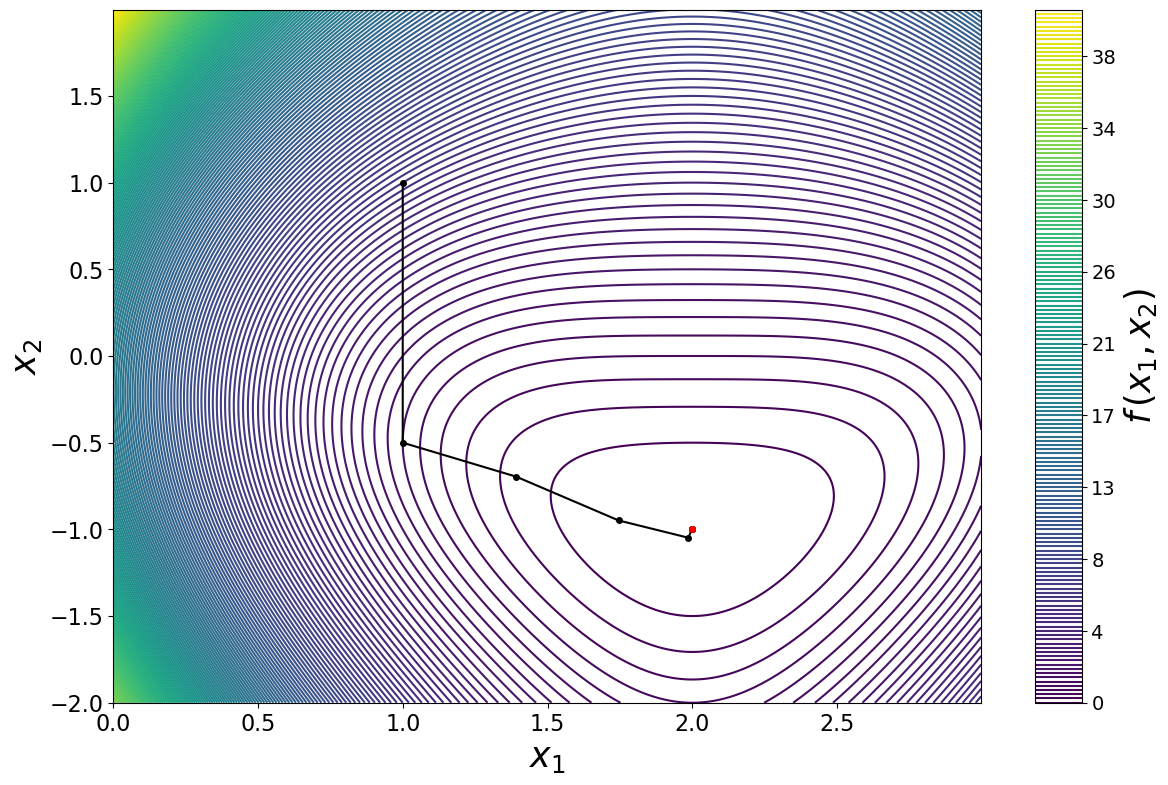
\includegraphics[scale=0.26]{Plot/func_a_standard_newton_contour.png}} \quad
		\subfloat[][]{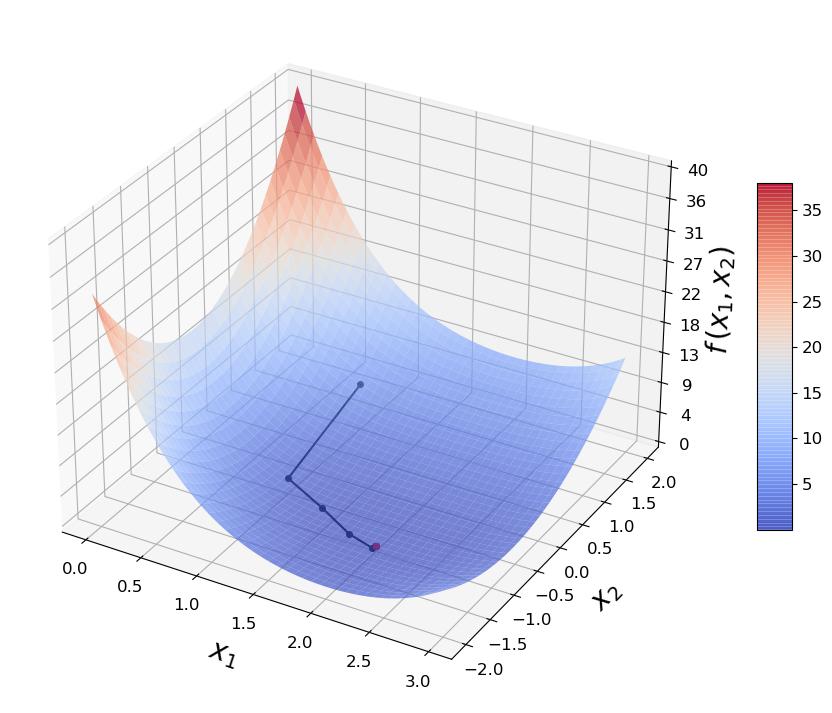
\includegraphics[scale=0.35]{Plot/func_a_standard_newton_3d.png}}
		\caption{Contour plot (Panel (a)) and 3D plot (Panel (b)) of the function $f^{(a)}(x_{1},x_{2})$ where the intermediate points and the minimum point (in red) are obtained by using the standard Newton algorithm with $\alpha=1$, starting from the point $\textbf{x}_{0}=(1,1)^{T}$.}
		\label{Fig:func_a}
	\end{figure}

	\noindent The second starting point which we consider is $\textbf{x}_{0}=(2,-1)^{T}$. This is exactly the minimum point of the function, therefore we expect the algorithm to converge in $0$ steps. The results that we obtain are the following:
	
\begin{minted}{text}
convergence = True, with 0 steps
min point = [ 2 -1]
min value = 0 
\end{minted}

	\subsection{Test function (b)}
	Consider the function $f^{(b)}:\mathbb{R}^{4} \rightarrow  \mathbb{R}$, defined as $f^{(b)}(\textbf{x}) = \textbf{b}^{T} + \frac{1}{2}\textbf{x}^{T}H\textbf{x}$, where:
	\begin{equation}
		\textbf{b} = (5.04, -59.4, 146.4, -96.6)^{T},
	\end{equation}

	\begin{equation}
		H = \begin{bmatrix}
		0.16 & -1.2 & 2.4 & -1.4 \\
		-1.2 & 12.0 & -27.0 & 16.8 \\
		2.4 & -27.0 & 64.8 & -42.0 \\
		-1.4 & 16.8 & -42.0 & 28.0
		\end{bmatrix}.
	\end{equation}
\noindent We know that the minimum point is $\textbf{x}^*=(1,0,-1,2)^{T}$ and the minimum value of the function is $f^{(b)}(\textbf{x}^*)=-167.28$. Moreover, in this case we have that $\nabla f^{(b)}(\textbf{x}) = H\textbf{x} + \textbf{b}$ and $\nabla^2 f^{(b)}(\textbf{x}) = H$. Since this is a quadratic function, we expect the standard Newton algorithm to converge in $1$ step, regardless of the starting point. In this case, we consider as starting point $\textbf{x}_{0}=(-1,3,3,0)^{T}$ and the results that we obtain are the following:
	\begin{minted}{text}
convergence = True, with 2 steps
min point = [ 1.000e+00 -4.730e-13 -1.000e+00  2.000e+00]
min value = -167.28
	\end{minted}
Below is the table with the required quantities at each step of the algorithm.
\begin{table}[H]
	\centering
	\begin{tabular}{|c|c|c|c|}
		\hline
		k & $\| \textbf{x}_{k} - \textbf{x}^*\|_{2} $ & $f^{(b)}(\textbf{x}_{k}) - f^{(b)}(\textbf{x}^{*}) $ & $-\nabla f^{(b)}(\textbf{x}_{k})^{T}[\nabla^{2}f^{(b)}(\textbf{x}_{k})]^{-1} \nabla f^{(b)}(\textbf{x}_{k})$ \\
		\hline
		$0$ & $5.745$ & $5.223\times10^{2}$ & $-1.045\times10^{3}$ \\
		$1$ & $9.769\times10^{-13}$ & $2.842\times10^{-14}$ & $-9.948\times10^{-27}$ \\
		$2$ & $1.688\times10^{-13}$ & $0.000$ & $-2.005\times10^{-26}$ \\
		\hline
	\end{tabular}
	\caption{Table of data obtained using the standard Newton algorithm to minimize the function $f^{(b)}(\textbf{x})$ by using $\alpha=1$ and by considering as starting point $\textbf{x}_{0}=(-1,3,3,0)^{T}$.}
	\label{Tab:func_b}
\end{table}

	\noindent The second, in principle unexpected, step is due to the convergence criterion. Recall that we have chosen as tolerance parameter \mintinline{Python}{tol=1e-12} and we have requested that two successive points must be close \textit{enough}, where enough means that it must be satisfied the condition $\|\textbf{x}_{k} - \textbf{x}_{k-1} \|_2 \le tol(1+ \| \textbf{x}_{k}\|_{2})$.

	\subsection{Test function (c)}
	Consider the function $f:\mathbb{R}^{2} \rightarrow  \mathbb{R}$, defined as 
	\begin{equation}
		f^{(c)}(x_{1},x_{2}) = (1.5 - x_{1}(1-x_{2}))^2 + (2.25 - x_{1}(1-x_{2}^{2}))^2 + (2.625 - x_{1}(1-x_{2}^{3}))^2.
	\end{equation}
	This function assumes a minimum value $f^{(c)}(\textbf{x}^*)=0$ in correspondence with the point $\textbf{x}^* = (3,0.5)^{T}$. The gradient and the Hessian of this function can be obtained, by linearity, by computing the gradient and the Hessian of each of the three terms in the expression of $f^{(c)}(\textbf{x})$ and then summing them up.\\
	
	\noindent We would like to obtain the minimum point and the minimum value of the function by using, as a first attempt, the standard Newton algorithm.\\
	
	 
	\noindent The first point that we consider is $\textbf{x}_{0}=(8,0.2)^{T}$. The results that we obtain are the following:
	
\begin{minted}{text}
convergence = True, with 9 steps
min point = [3.  0.5]
min value = 0.0
\end{minted}
We report in Tab \ref*{tab:table_c_x0_1} the required quantities at each step of the algorithm.
\begin{table}[H]
	\centering
	\begin{tabular}{|c|c|c|c|}
		\hline
		k & $\| \textbf{x}_{k} - \textbf{x}^*\|_{2} $ & $f^{(c)}(\textbf{x}_{k}) - f^{(c)}(\textbf{x}^{*}) $ & $-\nabla f^{(c)}(\textbf{x}_{k})^{T}[\nabla^{2}f^{(c)}(\textbf{x}_{k})]^{-1} \nabla f^{(c)}(\textbf{x}_{k})$ \\
		\hline
		$0$ & $5.009$ & $8.17\times10^{1}$ & $-1.455\times10^{2}$ \\
		$1$ & $8.66\times10^{-1}$ & $2.423$ & $-4.527$ \\
		$2$ & $6.494\times10^{-2}$ & $2.407\times10^{-2}$ & $-4.643\times10^{-2}$ \\
		$3$ & $1.393\times10^{-1}$ & $3.45\times10^{-3}$ & $-6.32\times10^{-3}$ \\
		$4$ & $2.103\times10^{-2}$ & $1.383\times10^{-4}$ & $-2.704\times10^{-4}$ \\
		$5$ & $1.377\times10^{-3}$ & $2.863\times10^{-7}$ & $-5.717\times10^{-7}$ \\
		$6$ & $3.033\times10^{-6}$ & $2.186\times10^{-12}$ & $-4.372\times10^{-12}$ \\
		$7$ & $2.836\times10^{-11}$ & $1.233\times10^{-22}$ & $-2.466\times10^{-22}$ \\
		$8$ & $4.441\times10^{-16}$ & $4.437\times10^{-31}$ & $-8.79\times10^{-31}$ \\
		$9$ & $0.000$ & $0.000$ & $0.000$ \\
		\hline
	\end{tabular}
	\caption{Table of data obtained using the standard Newton algorithm to minimize the function $f^{(c)}(x_{1},x_{2})$ by using $\alpha=1$ and by considering as starting point $\textbf{x}_{0}=(8,0.2)^{T}$.}
	\label{tab:table_c_x0_1}
\end{table}

	\begin{figure}[H]
		\centering
		\subfloat[][]{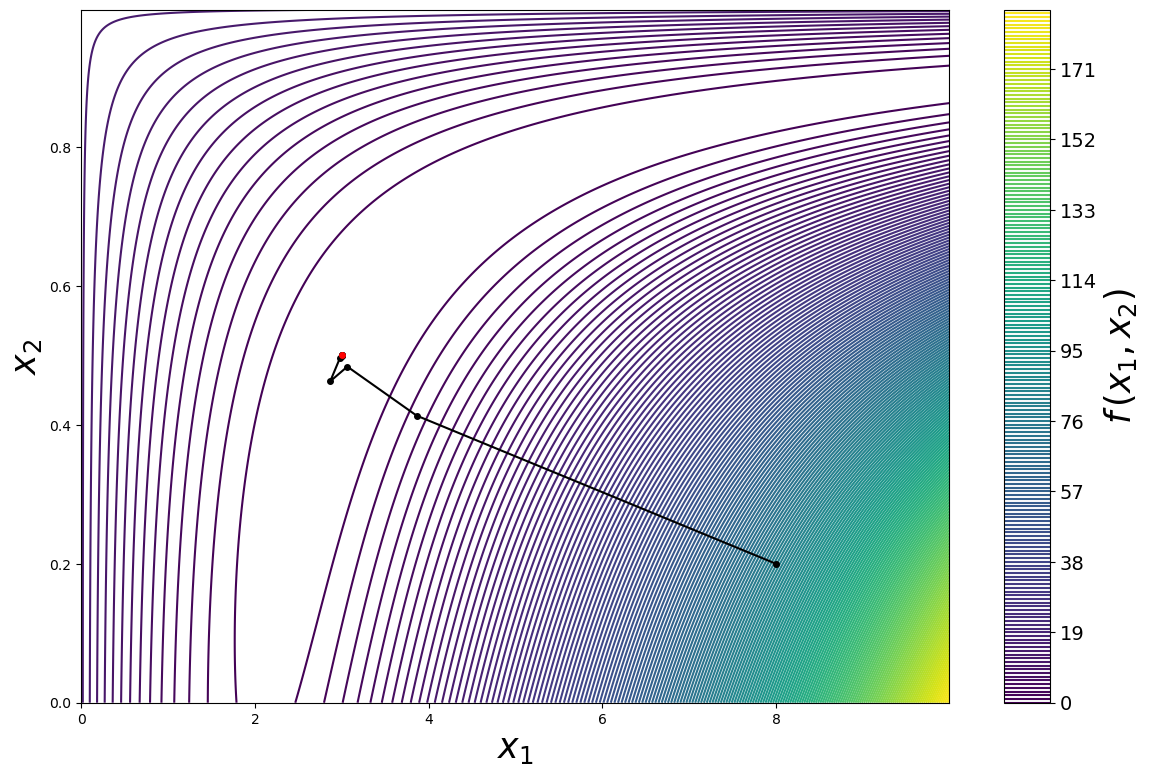
\includegraphics[scale=0.24]{Plot/func_c_standard_newton_x0_1_contour.png}} \quad
		\subfloat[][]{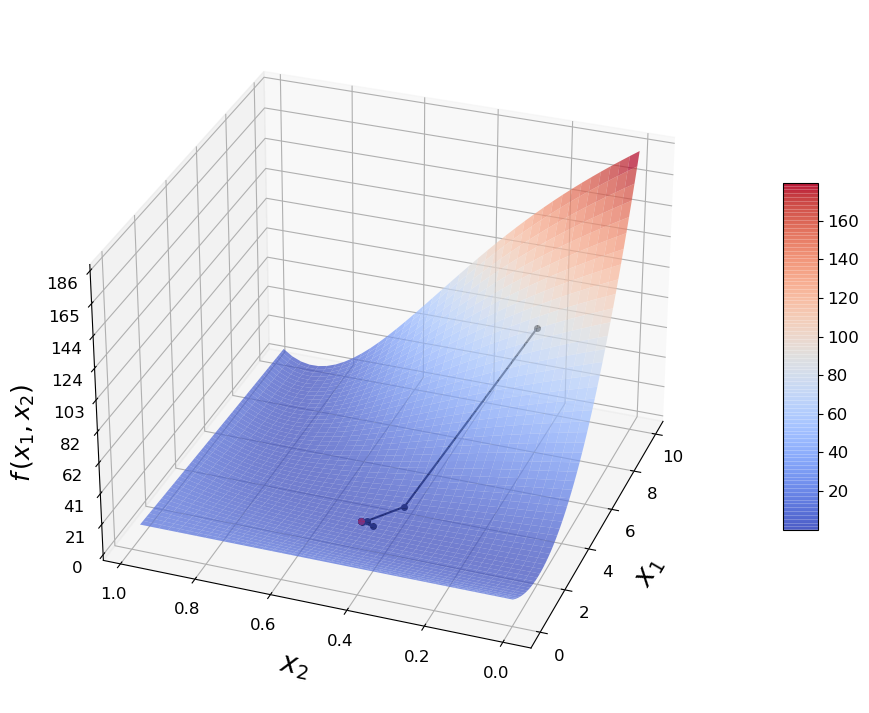
\includegraphics[scale=0.34]{Plot/func_c_standard_newton_x0_1_3d.png}}
		\caption{Contour plot (Panel (a)) and 3D plot (Panel (b)) of the function $f^{(c)}(x_{1},x_{2})$ where the intermediate points and the minimum point (in red) are obtained by using the standard Newton algorithm with $\alpha=1$, starting from the point $\textbf{x}_{0}=(8,0.2)^{T}$.}
		\label{Fig:func_c}
	\end{figure}

	\noindent As can be seen from the obtained results, the algorithm reaches convergence in $9$ step. This can be also seen by considering the quantities reported in Tab.~\ref{tab:table_c_x0_1} and the contour plot and the 3D plot reported in Fig.~\ref{Fig:func_c}.\\
	
	\noindent We now consider as starting point $\textbf{x}_{0}= (8,0.8)^{T}$. In this case, we obtain the following results:
	\begin{minted}{text}
convergence = True, with 10 steps
min point = [0. 1.]
min value = 14.203
	\end{minted}
As we can see, the algorithm converges in $10$ step to the point $\tilde{\textbf{x}}=(0,1)^{T}$ which, however, is not the minimum point of the function (which we know to be equal to $\textbf{x}^*=(3,0.5)^{T}$). This emerges also from the data reported in Tab.~\ref{tab:func_c_x0_2}, where one can see that the 2-norm of the difference between the computed point at step $k$ and the exact minimum point stabilizes to a non-zero value, as well as the difference between the value of the function at the point $\textbf{x}_{k}$ and the minimum value $f(\textbf{x}^*)$. What happens in this case is that the algorithm converges to a saddle point. In fact, at this point, the gradient of the function vanishes, i.e. $\nabla f^{(c)}(\tilde{\textbf{x}})=\textbf{0}$ (and this also reflects on the last points in Tab.~\ref{tab:func_c_x0_2}, since the scalar product between the gradient and the descent direction becomes equal to zero), while the Hessian is indefinite.
	\begin{table}[H]
		\centering
		\begin{tabular}{|c|c|c|c|}
			\hline
			k & $\| \textbf{x}_{k} - \textbf{x}^*\|_{2} $ & $f^{(c)}(\textbf{x}_{k}) - f^{(c)}(\textbf{x}^{*}) $ & $-\nabla f^{(c)}(\textbf{x}_{k})^{T}[\nabla^{2}f^{(c)}(\textbf{x}_{k})]^{-1} \nabla f^{(c)}(\textbf{x}_{k})$ \\
			\hline
			$0$ & $5.009$ & $2.043$ & $-3.291$ \\
			$1$ & $3.963$ & $2.553\times10^{-1}$ & $-5.885\times10^{-2}$ \\
			$2$ & $4.218$ & $2.328\times10^{-1}$ & $-6.421\times10^{-1}$ \\
			$3$ & $1.661\times10^{1}$ & $5.743\times10^{2}$ & $-9.291\times10^{2}$ \\
			$4$ & $6.137$ & $5.226\times10^{1}$ & $-6.327\times10^{1}$ \\
			$5$ & $3.426$ & $1.596\times10^{1}$ & $-3.709$ \\
			$6$ & $2.974$ & $1.421\times10^{1}$ & $-8.445\times10^{-3}$ \\
			$7$ & $3.041$ & $1.42\times10^{1}$ & $-5.688\times10^{-8}$ \\
			$8$ & $3.041$ & $1.42\times10^{1}$ & $-1.083\times10^{-18}$ \\
			$9$ & $3.041$ & $1.42\times10^{1}$ & $0.000$ \\
			$10$ & $3.041$ & $1.42\times10^{1}$ & $0.000$ \\
			\hline
		\end{tabular}
		\caption{Table of data obtained using the standard Newton algorithm to minimize the function $f^{(c)}(x_{1},x_{2})$ by using $\alpha=1$ and by considering as starting point $\textbf{x}_{0}=(8,0.8)^{T}$.}
		\label{tab:func_c_x0_2}
	\end{table}
	
	\begin{figure}[htb]
		\centering
		\subfloat[][]{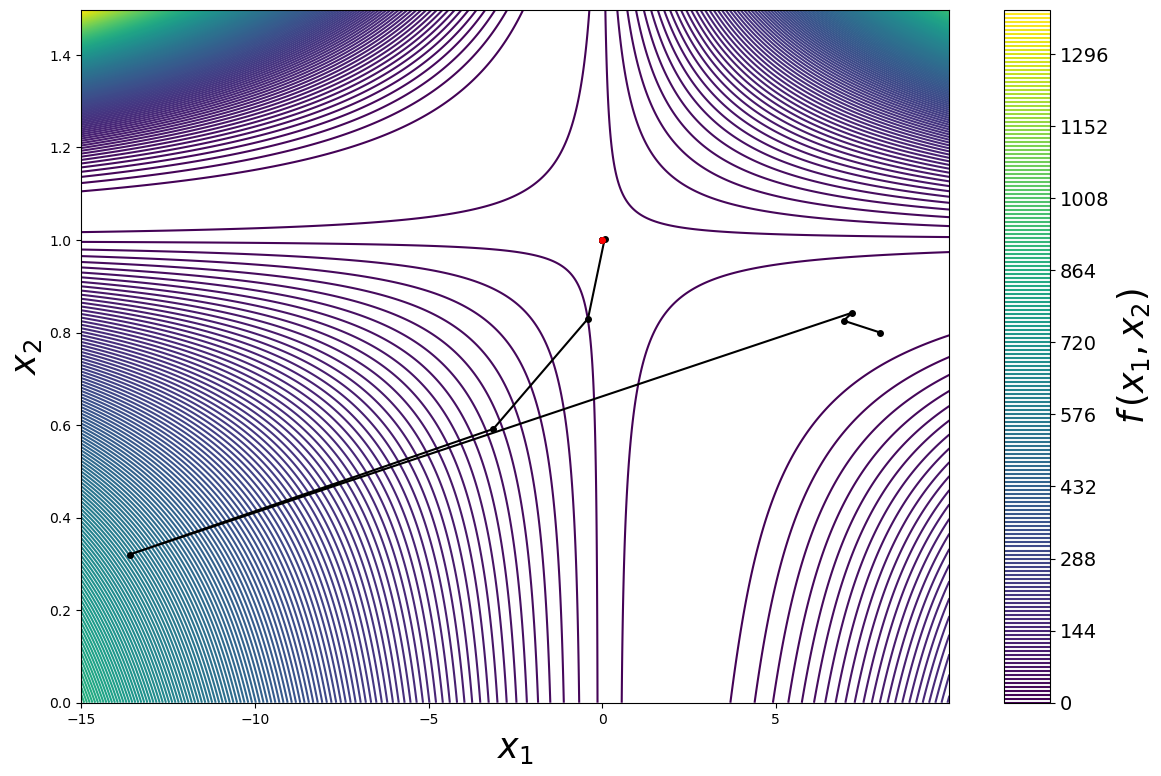
\includegraphics[scale=0.24]{Plot/func_c_standard_newton_x0_2_contour.png}} \quad
		\subfloat[][]{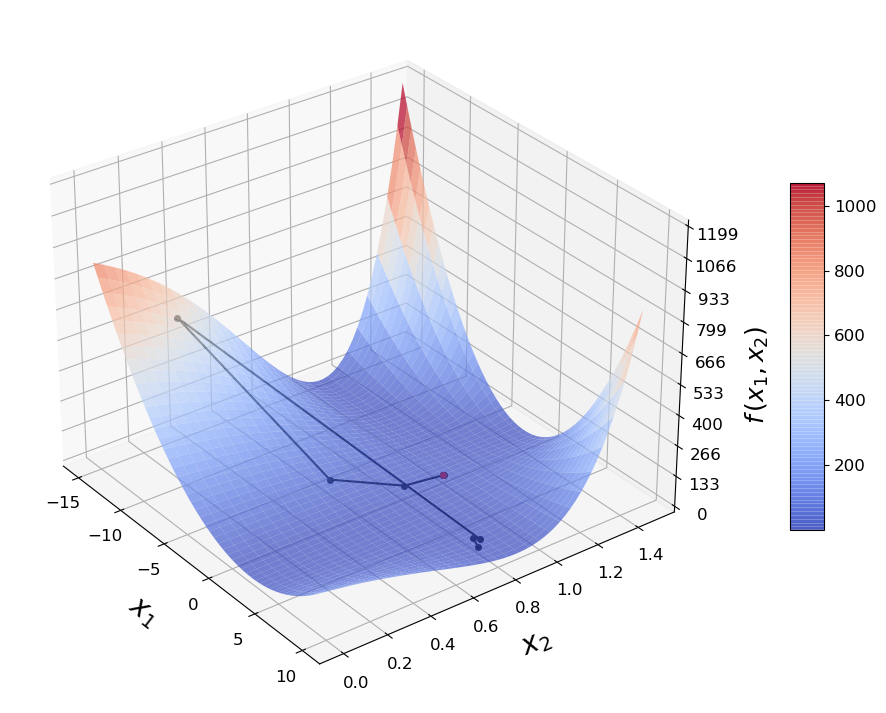
\includegraphics[scale=0.34]{Plot/func_c_standard_newton_x0_2_3d.png}}
		\caption{Contour plot (Panel (a)) and 3D plot (Panel (b)) of the function $f^{(c)}(x_{1},x_{2})$ where the intermediate points and the minimum point (in red) are obtained by using the standard Newton algorithm with $\alpha=1$, starting from the point $\textbf{x}_{0}=(8,0.8)^{T}$.}
		\label{Fig:func_c_x0_2}
	\end{figure}

\noindent To solve this problem, we tried to minimize the function $f^{(c)}(x_{1},x_{2})$ by using the Newton algorithm with backtracking, thanks to which it is possible to adapt the value of the step length $\alpha$ at each step. In this case, we obtain:
	\begin{minted}{text}
convergence = True, with 14 steps
min point = [3.  0.5]
min value = 0.0
	\end{minted}
We can see that the algorithm converges to the expected minimum point in $14$ steps. We report in Tab.~\ref{Tab:table_c_x0_2_backtracking} the required quantities at each step and in Fig.~\ref{Fig:func_c_x0_2_backtracking} the obtained contour plot and the 3D plot.

	\begin{table}[H]
		\centering
		\begin{tabular}{|c|c|c|c|}
			\hline
			k & $\| \textbf{x}_{k} - \textbf{x}^*\|_{2} $ & $f^{(c)}(\textbf{x}_{k}) - f^{(c)}(\textbf{x}^{*}) $ & $-\nabla f^{(c)}(\textbf{x}_{k})^{T}[\nabla^{2}f^{(c)}(\textbf{x}_{k})]^{-1} \nabla f^{(c)}(\textbf{x}_{k})$ \\
			\hline
			$0$ & $5.009$ & $2.043$ & $-3.291$ \\
			$1$ & $3.963$ & $2.553\times10^{-1}$ & $-5.885\times10^{-2}$ \\
			$2$ & $4.218$ & $2.328\times10^{-1}$ & $-6.421\times10^{-1}$ \\
			$3$ & $2.920$ & $2.131\times10^{-1}$ & $-7.337\times10^{-2}$ \\
			$4$ & $2.471$ & $1.649\times10^{-1}$ & $-1.224\times10^{-1}$ \\
			$5$ & $1.340$ & $1.502\times10^{-1}$ & $-1.22\times10^{-1}$ \\
			$6$ & $1.192$ & $7.989\times10^{-2}$ & $-1.697\times10^{-1}$ \\
			$7$ & $6.453\times10^{-1}$ & $5.012\times10^{-2}$ & $-5.027\times10^{-2}$ \\
			$8$ & $3.335\times10^{-1}$ & $1.73\times10^{-2}$ & $-2.418\times10^{-2}$ \\
			$9$ & $8.357\times10^{-2}$ & $3.009\times10^{-3}$ & $-5.269\times10^{-3}$ \\
			$10$ & $2.128\times10^{-2}$ & $1.004\times10^{-4}$ & $-1.967\times10^{-4}$ \\
			$11$ & $2.767\times10^{-4}$ & $1.503\times10^{-7}$ & $-3.005\times10^{-7}$ \\
			$12$ & $1.103\times10^{-6}$ & $2.293\times10^{-13}$ & $-4.585\times10^{-13}$ \\
			$13$ & $2.404\times10^{-13}$ & $8.166\times10^{-25}$ & $-1.633\times10^{-24}$ \\
			$14$ & $0.000$ & $0.000$ & $0.000$ \\
			\hline
		\end{tabular}
		\caption{Table of data obtained using the Newton algorithm with backtracking to minimize the function $f^{(c)}(x_{1},x_{2})$ by using $\alpha=1$, $\sigma=10^{-4}$, $\rho=0.5$ and by considering as starting point $\textbf{x}_{0}=(8,0.8)^{T}$.}
		\label{Tab:table_c_x0_2_backtracking}
	\end{table}
	
	\begin{figure}[htb]
		\centering
		\subfloat[][]{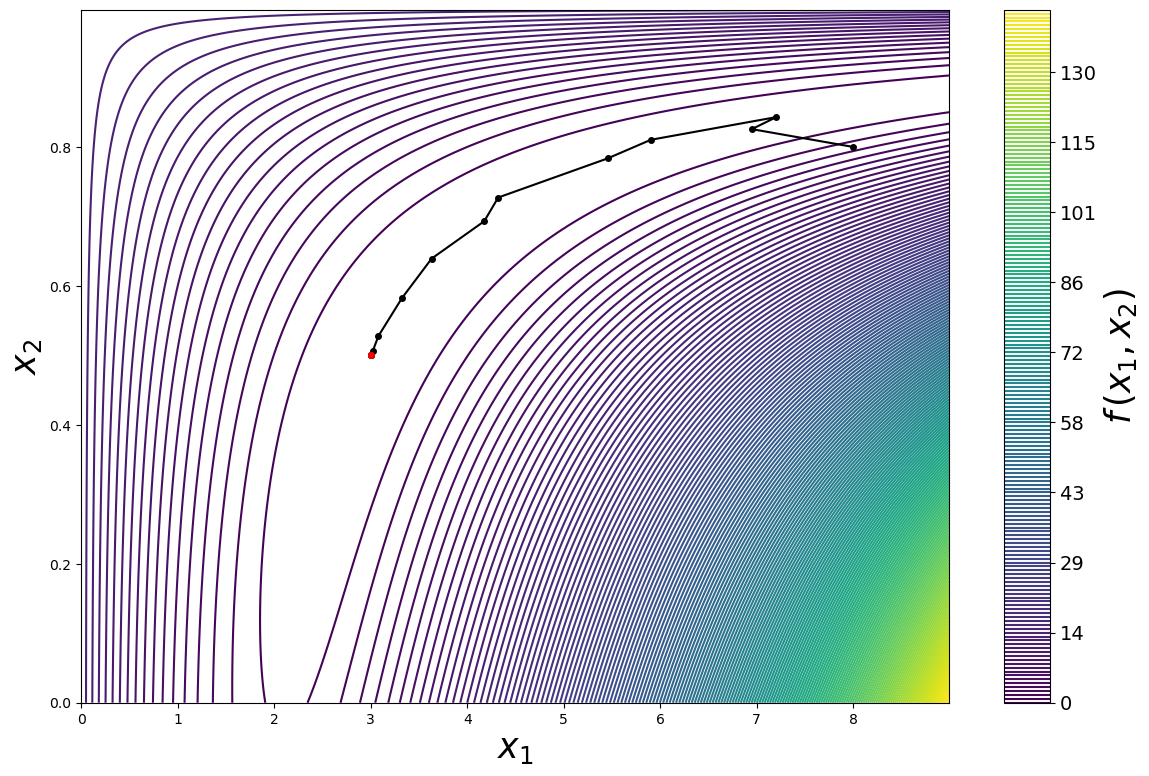
\includegraphics[scale=0.24]{Plot/func_c_standard_newton_backtrack_contour.png}} \quad
		\subfloat[][]{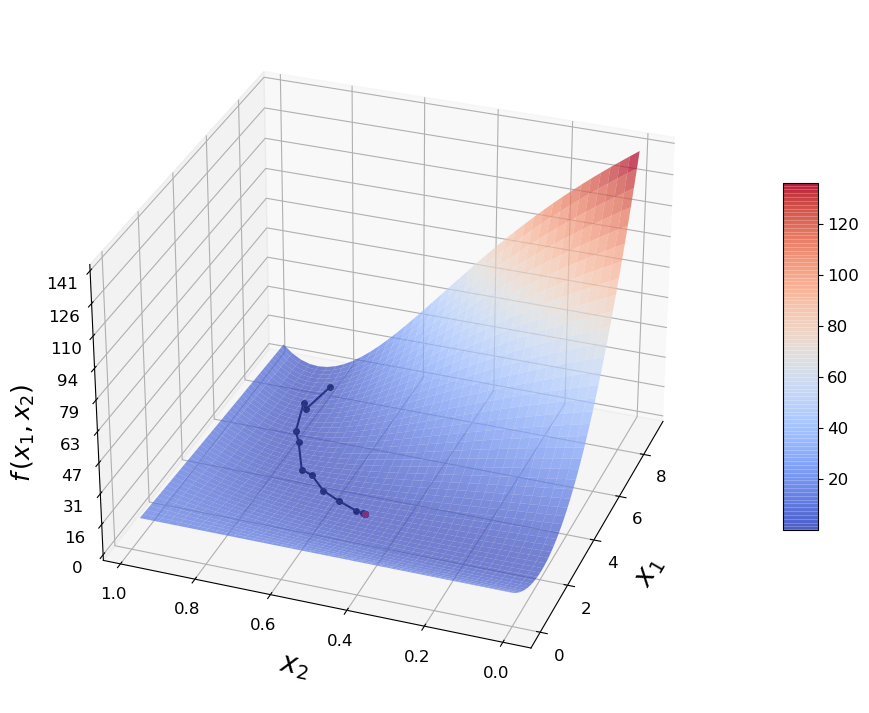
\includegraphics[scale=0.34]{Plot/func_c_standard_newton_backtrack_3d.png}}
		\caption{Contour plot (Panel (a)) and 3D plot (Panel (b)) of the function $f^{(c)}(x_{1},x_{2})$ where the intermediate points and the minimum point (in red) are obtained by using the Newton algorithm with backtracking, with $\alpha=1$, $\sigma=10^{-4}$, and $\rho=0.5$, starting from the point $\textbf{x}_{0}=(8,0.8)^{T}$.}
		\label{Fig:func_c_x0_2_backtracking}
	\end{figure}
	
	\subsection{Test function (d)}
	Consider the function $f:\mathbb{R}^{2} \rightarrow  \mathbb{R}$, defined as
	\begin{equation}
		f(x_{1},x_{2}) = x_{1}^{4} + x_{1}x_{2} + (1+x_{2})^{2}.
	\end{equation} This function assumes a minimum value $f^{(d)}(\textbf{x}^*)\simeq -0.582445174$ in correspondence with the point $\textbf{x}^{*}\simeq (0.695884386, -1.34794219)^{T}$. We report below the gradient and the Hessian of $f^{(d)}(\textbf{x})$, which must be passed as arguments to the Python function which performs the minimization.
	
	\begin{equation}
		\nabla f^{(d)}(\textbf{x}) = \begin{bmatrix}
			4x_{1}^{3} + x_{2} \\
			x_{1} +2(1+x_{2})
		\end{bmatrix}, \qquad \quad
		\nabla^2 f^{(d)}(\textbf{x}) = \begin{bmatrix}
		12x_{1}^{2} & 1 \\
		1 & 2
	\end{bmatrix}.
	\end{equation}

\noindent We consider first the starting point $\textbf{x}_{0}=(0.75,-1.25)^{T}$ and we try to see if the standard Newton algorithm converges, obtaining the following results:
\begin{minted}{text}
convergence = True, with 5 steps
min point = [ 0.69588439 -1.34794219]
min value = -0.5824451744436351
\end{minted}
In this case, the algorithm converges in $5$ steps. We report in Tab.~\ref{tab:table_d_x0_1} the required quantities and in Fig.~\ref{Fig:func_d_x0_1} the contour plot and the 3D plot.
	\begin{table}[H]
		\centering
		\begin{tabular}{|c|c|c|c|}
			\hline
			k & $\| \textbf{x}_{k} - \textbf{x}^*\|_{2} $ & $f^{(d)}(\textbf{x}_{k}) - f^{(d)}(\textbf{x}^{*}) $ & $-\nabla f^{(d)}(\textbf{x}_{k})^{T}[\nabla^{2}f^{(d)}(\textbf{x}_{k})]^{-1} \nabla f^{(d)}(\textbf{x}_{k})$ \\
			\hline
			$0$ & $1.119\times10^{-1}$ & $2.385\times10^{-2}$ & $-4.688\times10^{-2}$ \\
			$1$ & $4.601\times10^{-3}$ & $4.517\times10^{-5}$ & $-8.996\times10^{-5}$ \\
			$2$ & $2.951\times10^{-5}$ & $1.406\times10^{-9}$ & $-3.7\times10^{-9}$ \\
			$3$ & $3.805\times10^{-9}$ & $-4.436\times10^{-10}$ & $-6.372\times10^{-18}$ \\
			$4$ & $3.061\times10^{-9}$ & $-4.436\times10^{-10}$ & $0.000$ \\
			$5$ & $3.061\times10^{-9}$ & $-4.436\times10^{-10}$ & $0.000$ \\
			\hline
		\end{tabular}
		\caption{Table of data obtained using the standard Newton algorithm to minimize the function $f^{(d)}(x_{1},x_{2})$ by using $\alpha=1$ and by considering as starting point $\textbf{x}_{0}=(0.75,-1.25)^{T}$.}
		\label{tab:table_d_x0_1}
	\end{table}

	\begin{figure}[H]
		\centering
		\subfloat[][]{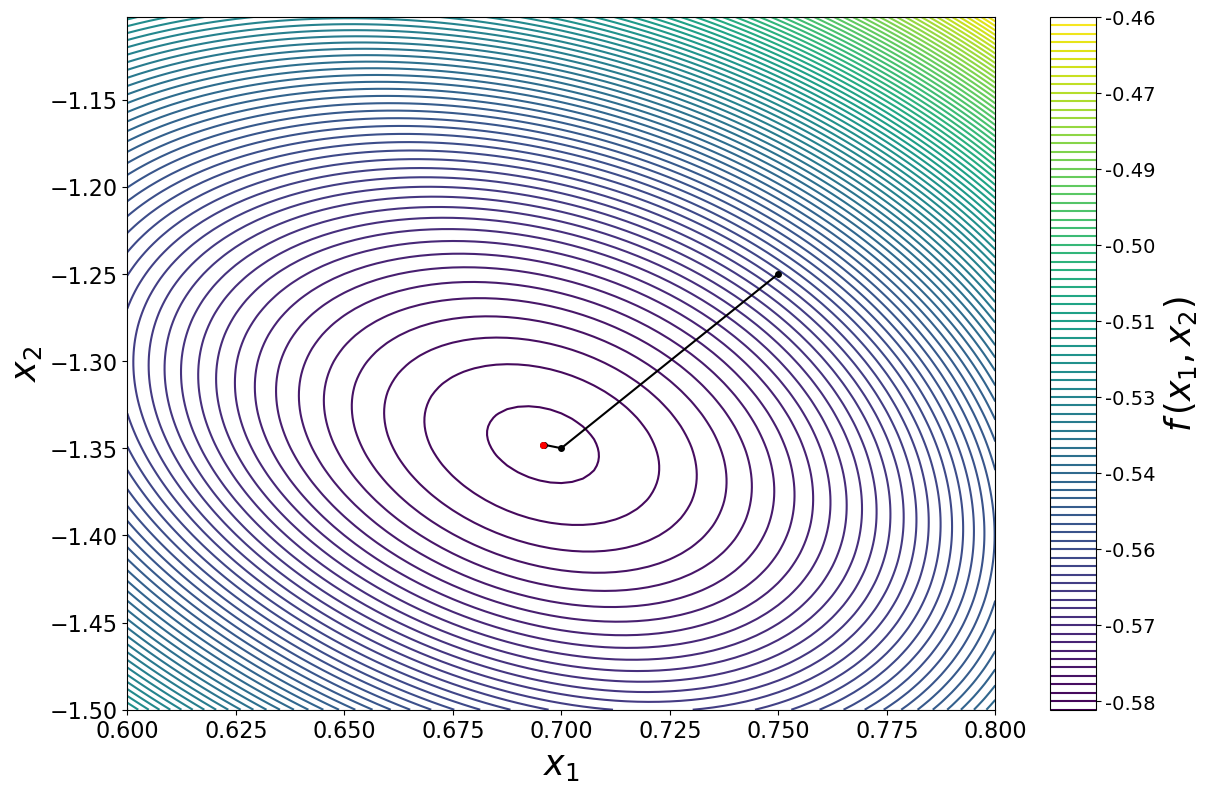
\includegraphics[scale=0.24]{Plot/func_d_standard_newton_x0_1_contour.png}} \quad
		\subfloat[][]{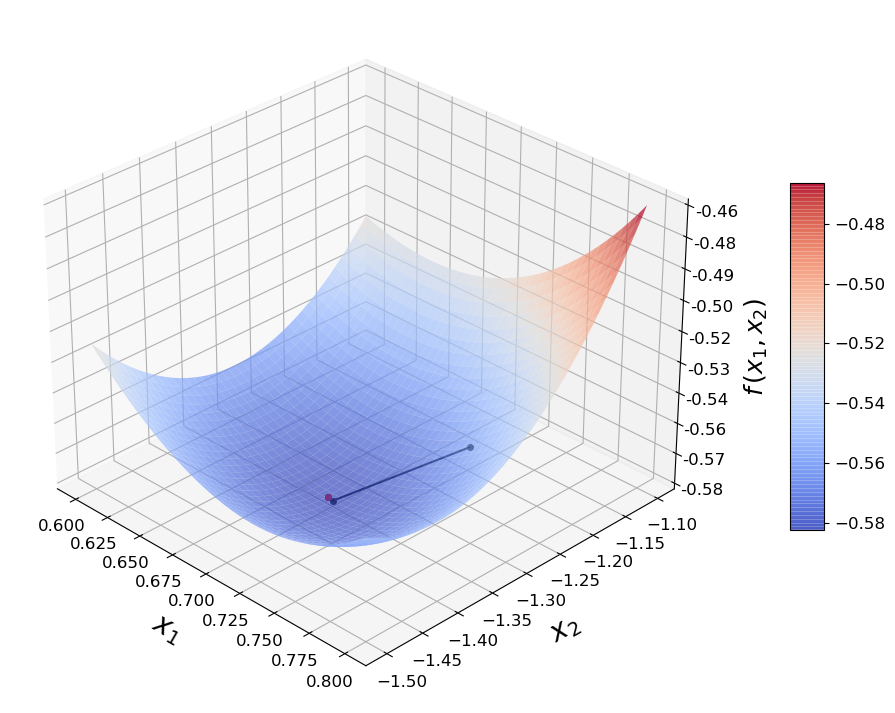
\includegraphics[scale=0.34]{Plot/func_d_standard_newton_x0_1_3d.png}}
		\caption{Contour plot (Panel (a)) and 3D plot (Panel (b)) of the function $f^{(d)}(x_{1},x_{2})$ where the intermediate points and the minimum point (in red) are obtained by using the standard Newton algorithm with $\alpha=1$, starting from the point $\textbf{x}_{0}=(0.75,-1.25)^{T}$.}
		\label{Fig:func_d_x0_1}
	\end{figure}

\noindent We now consider as starting point $\textbf{x}_{0}=(0,0)^{T}$. In this case, we can see that the standard Newton algorithm fails to converge, indeed
\begin{minted}{text}
convergence = False, with 100 steps
min point = [ 0.00169883 -1.00084941]
min value = -0.0016995470778935944
\end{minted}
As emerges from these results, after $100$ iterations the algorithm does not reach the minimum point of the considered function. We report in Tab.~\ref{tab:func_d_x0_2} the first and the last values of the required quantities.
\begin{table}[H]
	\centering
	\begin{tabular}{|c|c|c|c|}
		\hline
		k & $\| \textbf{x}_{k} - \textbf{x}^*\|_{2} $ & $f^{(d)}(\textbf{x}_{k}) - f^{(d)}(\textbf{x}^{*}) $ & $-\nabla f^{(d)}(\textbf{x}_{k})^{T}[\nabla^{2}f^{(d)}(\textbf{x}_{k})]^{-1} \nabla f^{(d)}(\textbf{x}_{k})$ \\
		\hline
		$0$ & $1.517$ & $1.582$ & $0.000$ \\
		$1$ & $3.014$ & $1.758\times10^{1}$ & $-2.156\times10^{1}$ \\
		$2$ & $2.261$ & $4.563$ & $-4.537$ \\
		$3$ & $1.736$ & $1.796$ & $-1.148$ \\
		$4$ & $1.321$ & $1.065$ & $-6.339\times10^{-1}$ \\
		$5$ & $7.376\times10^{-1}$ & $5.459\times10^{-1}$ & $2.140$ \\
		$6$ & $3.088$ & $1.979\times10^{1}$ & $-2.447\times10^{1}$ \\
		$7$ & $2.311$ & $5.017$ & $-5.116$ \\
		$8$ & $1.772$ & $1.900$ & $-1.262$ \\
		$9$ & $1.353$ & $1.101$ & $-6.193\times10^{-1}$ \\
		$10$ & $8.159\times10^{-1}$ & $6.16\times10^{-1}$ & $1.988$ \\
		$11$ & $3.077$ & $1.945\times10^{1}$ & $-2.402\times10^{1}$ \\
		\vdots & \vdots &  \vdots & \vdots \\
		$90$ & $7.939\times10^{-1}$ & $5.966\times10^{-1}$ & $1.981$ \\
		$91$ & $3.025$ & $1.789\times10^{1}$ & $-2.197\times10^{1}$ \\
		$92$ & $2.268$ & $4.627$ & $-4.618$ \\
		$93$ & $1.742$ & $1.810$ & $-1.164$ \\
		$94$ & $1.326$ & $1.070$ & $-6.309\times10^{-1}$ \\
		$95$ & $7.501\times10^{-1}$ & $5.573\times10^{-1}$ & $2.081$ \\
		$96$ & $3.048$ & $1.859\times10^{1}$ & $-2.288\times10^{1}$ \\
		$97$ & $2.284$ & $4.770$ & $-4.800$ \\
		$98$ & $1.753$ & $1.843$ & $-1.200$ \\
		$99$ & $1.336$ & $1.082$ & $-6.254\times10^{-1}$ \\
		$100$ & $7.761\times10^{-1}$ & $5.807\times10^{-1}$ & $2.004$ \\
		\hline
	\end{tabular}
	\caption{Table of data obtained using the standard Newton algorithm to minimize the function $f^{(d)}(x_{1},x_{2})$ by using $\alpha=1$ and by considering as starting point $\textbf{x}_{0}=(0,0)^{T}$.}
	\label{tab:func_d_x0_2}
\end{table}
\noindent From these results, we can see that the 2-norm of the difference between the computed point at step $k$ and the exact minimum point decreases every five iterations and then increases again, and this also happens when considering the difference between $f^{(d)}(\textbf{x}_{k})$ and  $f^{(d)}(\textbf{x}^*)$. This suggests that the computed point tries to slowly approach the exact minimum point but then moves away again, showing a sort of zig-zag pattern. In fact, if we consider the scalar product between the gradient of the function and the descent direction we can observe that at the fifth iteration, and every five iterations, it becomes positive, suggesting that in the next step the new point will move away from the minimum point. A possible explanation of this behavior might be that the value of $\alpha$ is too large.\\

\noindent To reach convergence we have first tried to use the standard Newton algorithm considering a different value for $\alpha$. In particular, we observe that it is possible to reach convergence by choosing $\alpha=0.9$ instead of $\alpha=1$.
\begin{minted}{text}
convergence = True, with 25 steps
min point = [ 0.69588439 -1.34794219]
min value = -0.5824451744436351
\end{minted}
From these results we can see that the computed minimum point and the computed minimum value of the function coincide with the exact ones. However, in this case, the number of iterations required to reach convergence is $25$, and one might be tempted to improve this result by using a different method.
	\begin{table}[H] 
		\centering 
		\begin{tabular}{|c|c|c|c|} 
			\hline 
			k & $\| \textbf{x}_{k} - \textbf{x}^*\|_{2} $ & $f^{(d)}(\textbf{x}_{k}) - f^{(d)}(\textbf{x}^{*}) $ & $-\nabla f^{(d)}(\textbf{x}_{k})^{T}[\nabla^{2}f^{(d)}(\textbf{x}_{k})]^{-1} \nabla f^{(d)}(\textbf{x}_{k})$ \\
			\hline
			$0$ & $1.517$ & $1.582$ & $0.000$ \\
			$1$ & $2.837$ & $1.208\times10^{1}$ & $-1.432\times10^{1}$ \\
			$2$ & $2.181$ & $3.888$ & $-3.680$ \\
			$3$ & $1.725$ & $1.764$ & $-1.114$ \\
			$4$ & $1.352$ & $1.099$ & $-6.198\times10^{-1}$ \\
			$5$ & $8.656\times10^{-1}$ & $6.593\times10^{-1}$ & $2.174$ \\
			$6$ & $3.138$ & $2.143\times10^{1}$ & $-2.663\times10^{1}$ \\
			$7$ & $2.424$ & $6.213$ & $-6.657$ \\
			$8$ & $1.910$ & $2.391$ & $-1.830$ \\
			$9$ & $1.514$ & $1.320$ & $-6.987\times10^{-1}$ \\
			$10$ & $1.126$ & $8.791\times10^{-1}$ & $-1.402$ \\
			$11$ & $3.352\times10^{-1}$ & $3.219\times10^{-1}$ & $-5.271\times10^{-1}$ \\
			$12$ & $1.188\times10^{-1}$ & $3.348\times10^{-2}$ & $-6.1\times10^{-2}$ \\
			$13$ & $2.637\times10^{-2}$ & $1.514\times10^{-3}$ & $-2.957\times10^{-3}$ \\
			$14$ & $3.474\times10^{-3}$ & $2.572\times10^{-5}$ & $-5.128\times10^{-5}$ \\
			$15$ & $3.626\times10^{-4}$ & $2.789\times10^{-7}$ & $-5.586\times10^{-7}$ \\
			$16$ & $3.643\times10^{-5}$ & $2.375\times10^{-9}$ & $-5.637\times10^{-9}$ \\
			$17$ & $3.646\times10^{-6}$ & $-4.154\times10^{-10}$ & $-5.642\times10^{-11}$ \\
			$18$ & $3.659\times10^{-7}$ & $-4.434\times10^{-10}$ & $-5.643\times10^{-13}$ \\
			$19$ & $3.801\times10^{-8}$ & $-4.436\times10^{-10}$ & $-5.643\times10^{-15}$ \\
			$20$ & $5.778\times10^{-9}$ & $-4.436\times10^{-10}$ & $-5.643\times10^{-17}$ \\
			$21$ & $3.252\times10^{-9}$ & $-4.436\times10^{-10}$ & $-5.643\times10^{-19}$ \\
			$22$ & $3.079\times10^{-9}$ & $-4.436\times10^{-10}$ & $-5.643\times10^{-21}$ \\
			$23$ & $3.063\times10^{-9}$ & $-4.436\times10^{-10}$ & $-5.643\times10^{-23}$ \\
			$24$ & $3.061\times10^{-9}$ & $-4.436\times10^{-10}$ & $-5.644\times10^{-25}$ \\
			$25$ & $3.061\times10^{-9}$ & $-4.436\times10^{-10}$ & $-5.63\times10^{-27}$ \\
			\hline
		\end{tabular}
		\caption{Table of data obtained using the standard Newton algorithm to minimize the function $f^{(d)}(x_{1},x_{2})$ by using $\alpha=0.9$ and by considering as starting point $\textbf{x}_{0}=(0,0)^{T}$.}
	\end{table}
	
	\begin{figure}[H]
		\centering
		\subfloat[][]{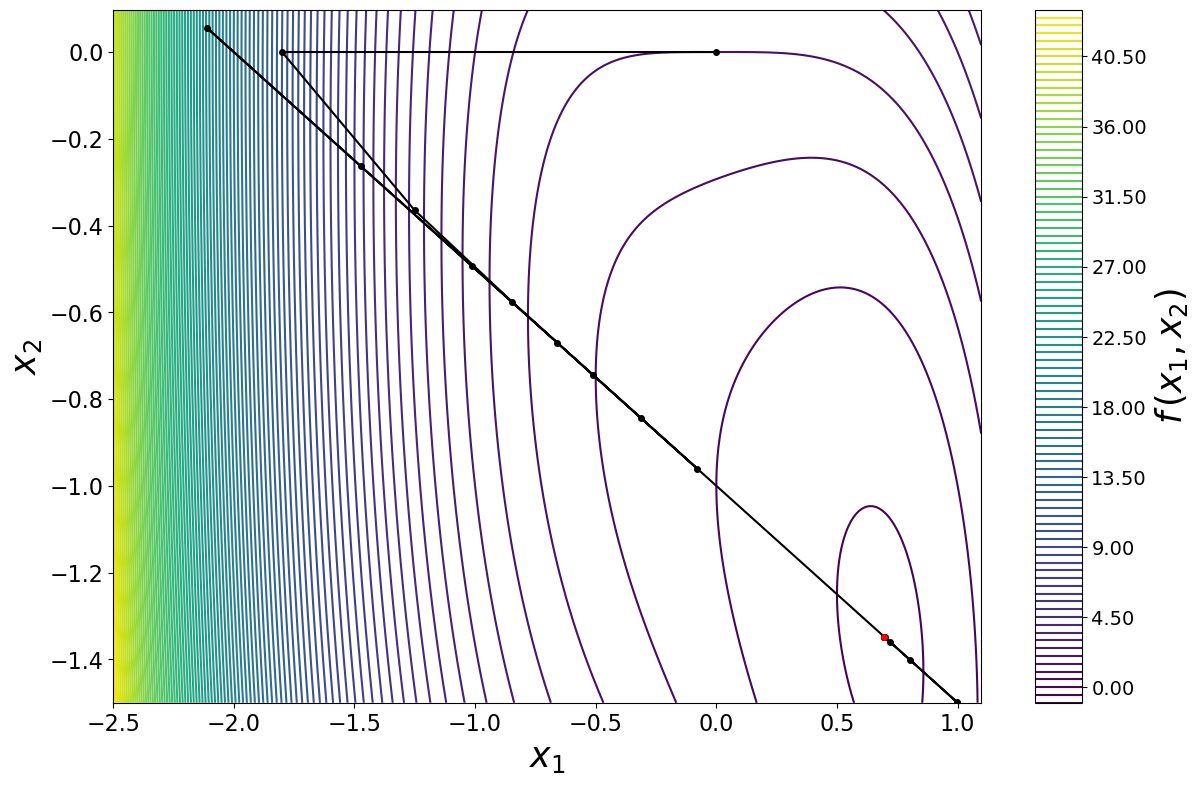
\includegraphics[scale=0.24]{Plot/func_d_standard_newton_x0_2_alpha=0.9_contour.png}} \quad
		\subfloat[][]{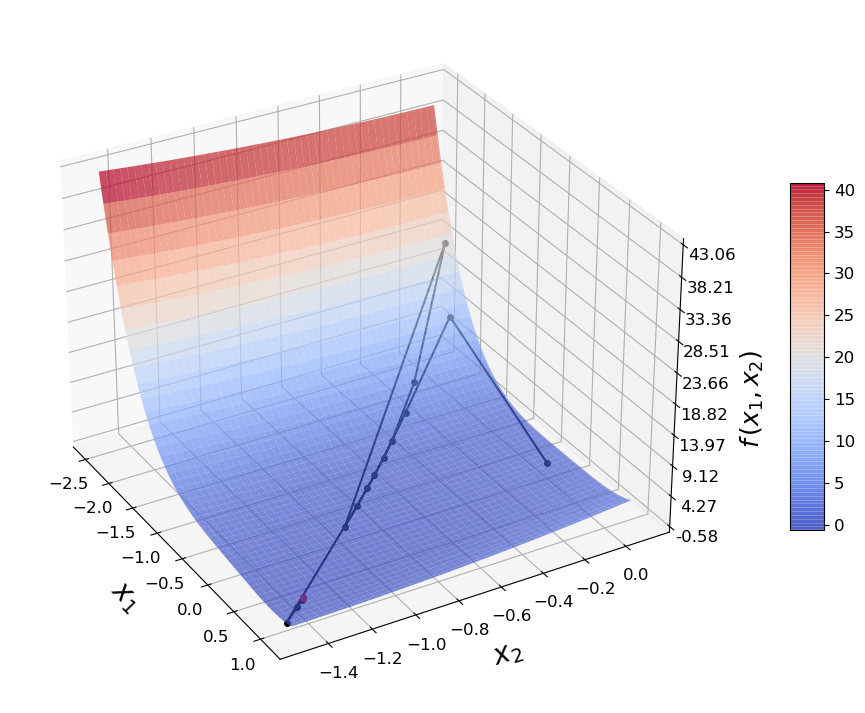
\includegraphics[scale=0.34]{Plot/func_d_standard_newton_x0_2_alpha=0.9_3d.png}}
		\caption{Contour plot and 3D plot for the function $f^{(d)}(x_{1},x_{2})$ where the intermediate points and the minimum point (in red) are obtained by using the standard Newton method with $\alpha=0.9$, starting from the point $\textbf{x}_{0}=(0,0)^{T}$.}
		\label{Fig:func_d}
	\end{figure}

\noindent For this reason, we have implemented the trust region Newton algorithm to see if it is possible to reach convergence in fewer steps. In this case, we obtain the following results:
\begin{minted}{text}
convergence = True, with 8 steps
min point = [ 0.69588439 -1.34794219]
min value = -0.5824451744436351
\end{minted}
We can see that, in this case, the algorithm converges in $8$ steps, returning the expected minimum point and the corresponding minimum value of the function. We report in Tab.~\ref{tab:func_d_x0_2_trustreg} the required quantities at each step of the algorithm and in Fig.~\ref{Fig:func_d_x0_2_trustreg} the obtained contour plot and the 3D plot.

	\begin{table}[H]
		\centering
		\begin{tabular}{|c|c|c|c|}
			\hline
			k & $\| \textbf{x}_{k} - \textbf{x}^*\|_{2} $ & $f^{(d)}(\textbf{x}_{k}) - f^{(d)}(\textbf{x}^{*}) $ & $-\nabla f^{(d)}(\textbf{x}_{k})^{T}[\nabla^{2}f^{(d)}(\textbf{x}_{k})]^{-1} \nabla f^{(d)}(\textbf{x}_{k})$ \\
			\hline
			$0$ & $1.517$ & $1.582$ & $0.000$ \\
			$1$ & $8.014\times10^{-1}$ & $3.716$ & $-5.554$ \\
			$2$ & $3.959\times10^{-1}$ & $4.724\times10^{-1}$ & $-7.576\times10^{-1}$ \\
			$3$ & $1.232\times10^{-1}$ & $3.61\times10^{-2}$ & $-6.559\times10^{-2}$ \\
			$4$ & $1.717\times10^{-2}$ & $6.364\times10^{-4}$ & $-1.253\times10^{-3}$ \\
			$5$ & $4.011\times10^{-4}$ & $3.414\times10^{-7}$ & $-6.834\times10^{-7}$ \\
			$6$ & $2.275\times10^{-7}$ & $-4.435\times10^{-10}$ & $-2.171\times10^{-13}$ \\
			$7$ & $3.061\times10^{-9}$ & $-4.436\times10^{-10}$ & $-2.197\times10^{-26}$ \\
			$8$ & $3.061\times10^{-9}$ & $-4.436\times10^{-10}$ & $0.000$ \\
			\hline
		\end{tabular}
		\caption{Table of data obtained using the trust region Newton algorithm to minimize the function $f^{(d)}(x_{1},x_{2})$ by using $\alpha=1$ and $\eta=10^{-2}$ and by considering as starting point $\textbf{x}_{0}=(0,0)^{T}$.}
		\label{tab:func_d_x0_2_trustreg}
	\end{table}
	
		\begin{figure}[H]
		\centering
		\subfloat[][]{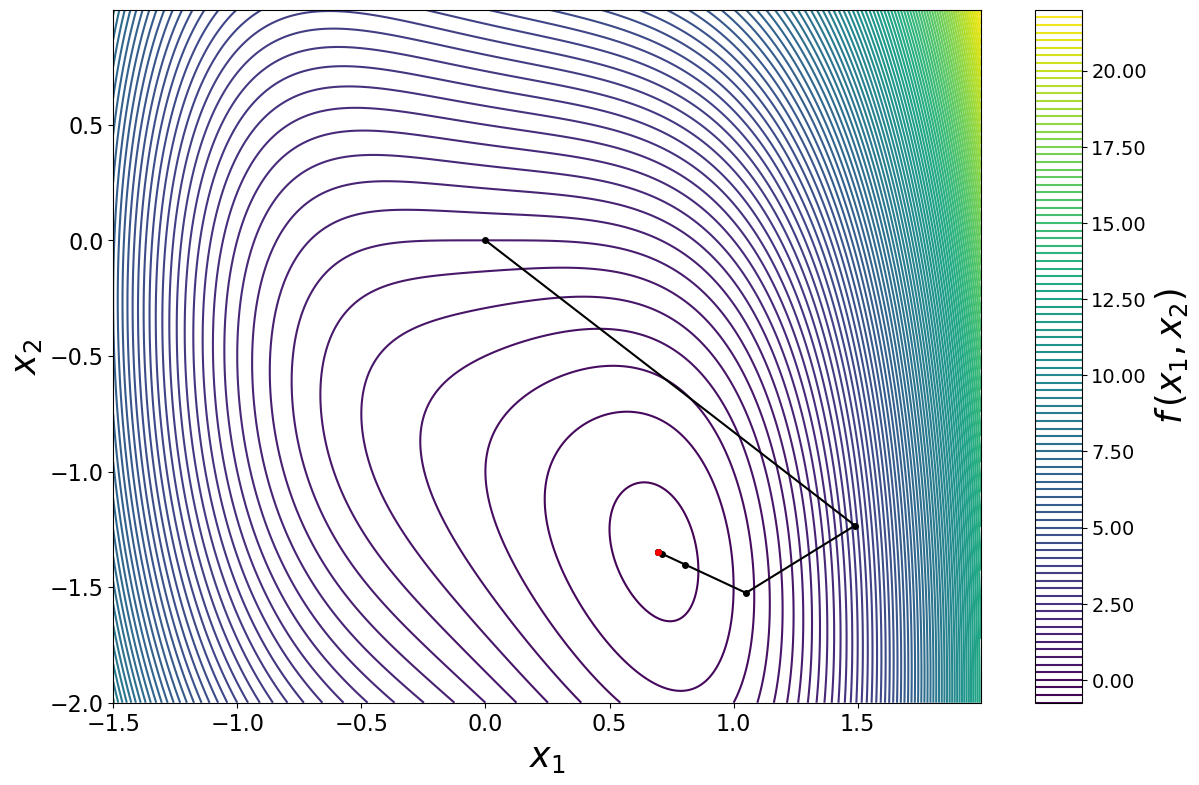
\includegraphics[scale=0.24]{Plot/func_d_newton_trustreg_contour.png}} \quad
		\subfloat[][]{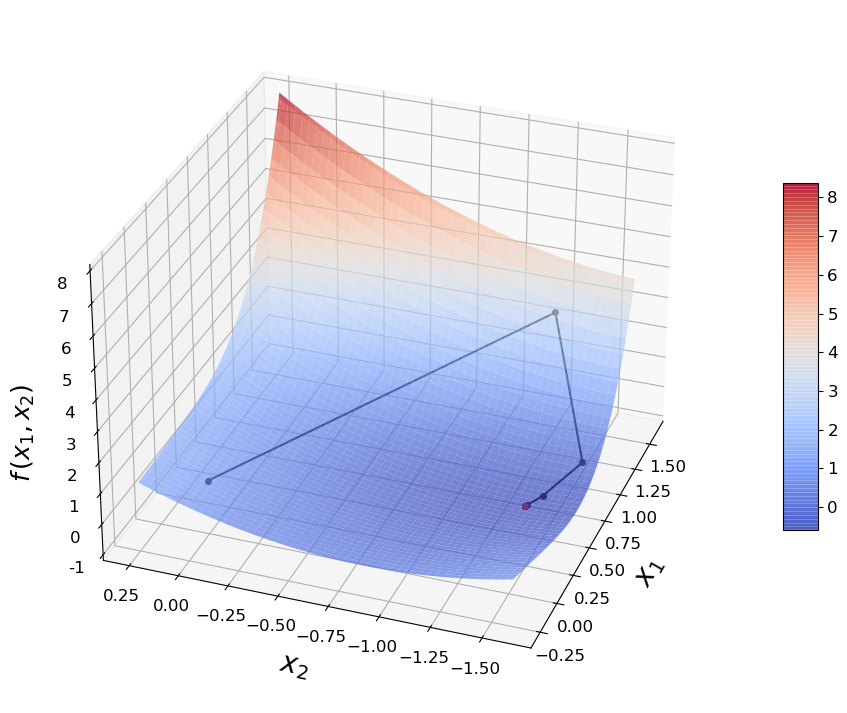
\includegraphics[scale=0.34]{Plot/func_d_newton_trustreg_3d.png}}
		\caption{Contour plot and 3D plot of the function $f^{(d)}(x_{1},x_{2})$ where the intermediate points and the minimum point (in red) are obtained by using the Newton method with the trust region approach with $\alpha=1$, $\eta=10^{-2}$, starting from the point $\textbf{x}_{0}=(0,0)^{T}$.}
		\label{Fig:func_d_x0_2_trustreg}
	\end{figure}
	
\end{document}